
\begin{enumerate}
	\item In the given figure \figref{fig:circle1}, $ PQ $ is tangent to the circle centred at $ \vec{O} $. If $ \angle{AOB} = 95{\degree} $, then measure of $ \angle{ABQ} $ will be
	\begin{figure}[H]
		\centering
		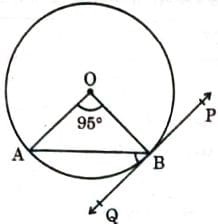
\includegraphics[width=\columnwidth]{figs/circle1.jpg}
		\caption{}
		\label{fig:circle1}
	\end{figure}
		\begin{enumerate}
			\item $ 47.5{\degree} $
			\item $ 42.5{\degree} $
			\item $ 85{\degree} $
			\item $ 95{\degree} $
		\end{enumerate}
	\item
		\begin{enumerate}
			\item In the given figure \figref{fig:circle2}, two tangents $ TP $ and $ TQ $ are drawn to be a circle with centre $ \vec{O} $ from an external point $ \vec{T} $. Prove that $ \angle{PTQ} = 2\angle{OPQ} $.
		\begin{figure}[H]
			\centering
			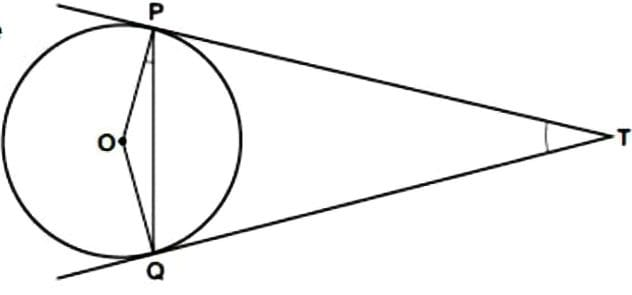
\includegraphics[width=\columnwidth]{figs/circle2.jpg}
			\caption{}
			\label{fig:circle2}
		\end{figure}
	\item In the given figure \figref{fig:circle3}, a circle is inscribed in a quadrilateral $ ABCD $ in which $ \angle{B} = 90{\degree} $. If $ AD = 17 cm, AB = 20 cm $ and $ DS = 3cm $, then find the radius of the circle.
		\begin{figure}[H]
			\centering 
			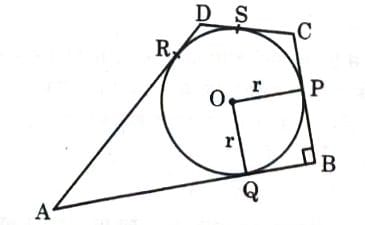
\includegraphics[width=\columnwidth]{figs/circle3.jpg}
			\caption{}
			\label{fig:circle3}
		\end{figure}
		\end{enumerate}
	\item The discus throw is an event in which an athlete attempts to throw a discus. The athlete spins anti-clockwise around one and a half times through a cicrle as shown in \figref{fig:tangentline} below, then releases the throw. When released, the discus travels along tangent to the circular spin orbit.
		\begin{figure}[H]
			\centering
			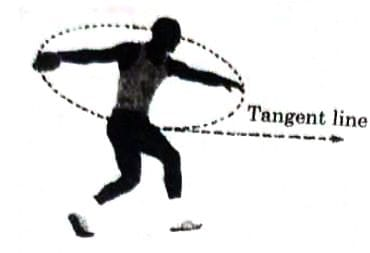
\includegraphics[width=\columnwidth]{figs/circle4.jpg}
			\caption{}
			\label{fig:tangentline}
		\end{figure}
		In the given figure \figref{fig:circle5}, $ AB $ is one such tangent to a circle of radius 75 cm. Point $ \vec{O} $ is centre of the circle and $ \angle{ABO} = 30{\degree} . PQ $ is parallel to $ OA $.
		\begin{figure}[H]
			\centering
			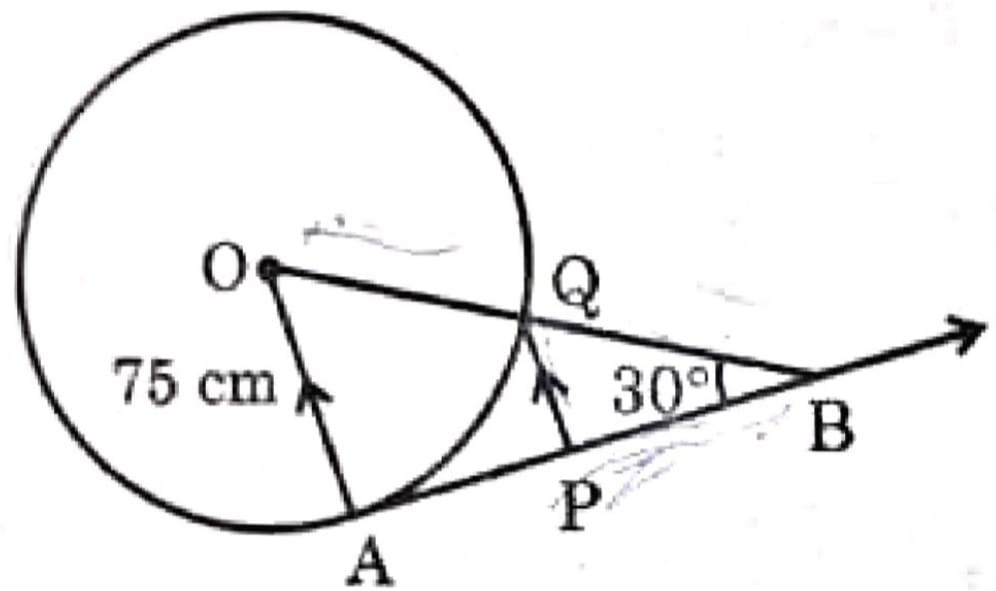
\includegraphics[width=\columnwidth]{figs/circle5.jpg}
			\caption{}
			\label{fig:circle5}
		\end{figure}
		Based on above information :
		\begin{enumerate}
			\item find the length of $ AB $.
			\item find the length of $ OB $.
			\item find the length of $ AP $.
			\item find the length of $ PQ $.
		\end{enumerate}
	\item In the given figure \figref{fig:circle6}, the quadrilateral $ PQRS $ circumscribes a circle. Here $ PA + CS $ is equal to :
		\begin{figure}[H]
			\centering
			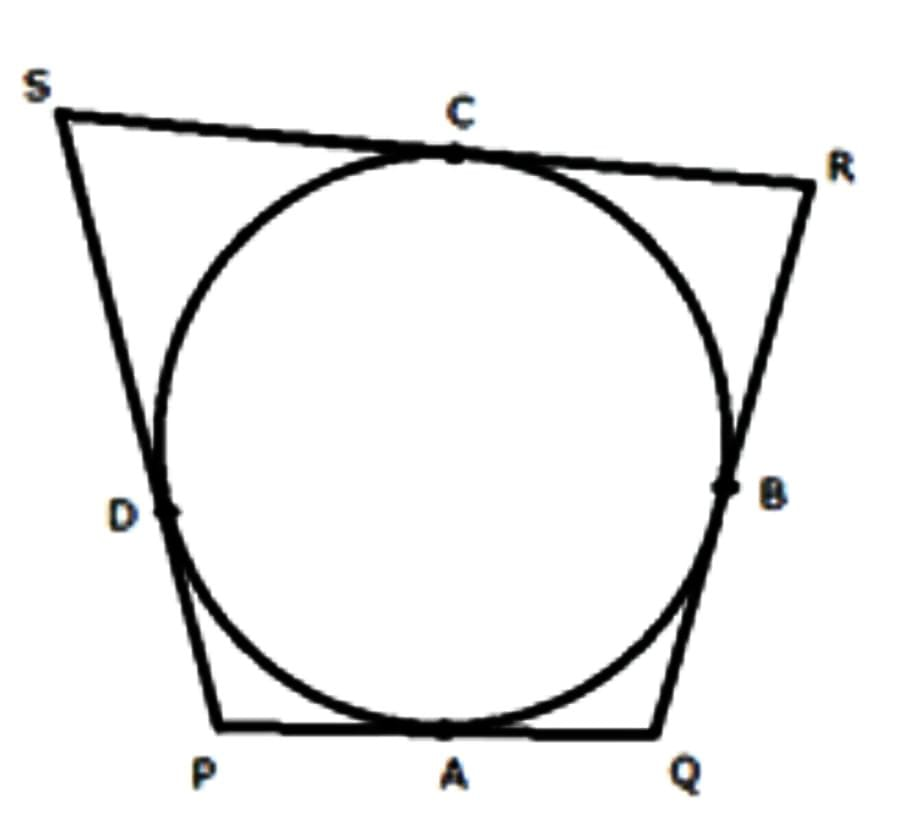
\includegraphics[width=\columnwidth]{figs/circle6.jpg}
			\caption{}
			\label{fig:circle6}
		\end{figure}
		\begin{enumerate}
			\item $ QR $
			\item $ PR $
			\item $ PS $
			\item $ PQ $
		\end{enumerate}
	\item In the given figure \figref{fig:circle7}, $ \vec{O} $ is the centre of the circle. $ AB $ and $ AC $ are tangents drawn to the circle from point $ \vec{A} $. If $ \angle{BAC} = 65{\degree} $, then find the measure of $ \angle{BOC} $.
		\begin{figure}[H]
			\centering
			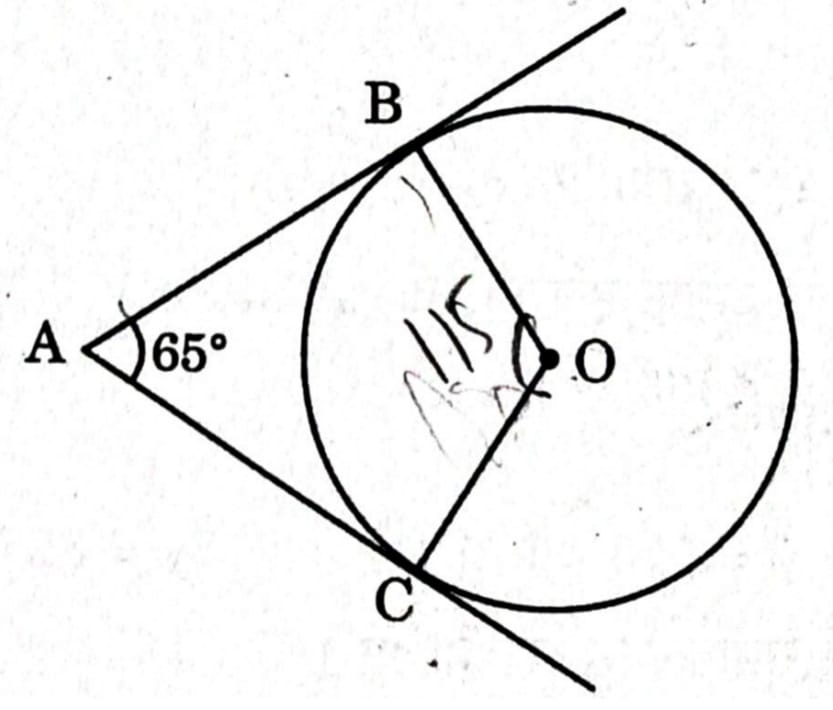
\includegraphics[width=\columnwidth]{figs/circle7.jpg}
			\caption{}
			\label{fig:circle7}
		\end{figure}
	\item In the given figure \figref{fig:circle8}, $ \vec{O} $ is the centre of the circle and $ QPR $ is the tangent to it at $ \vec{P} $. Prove that $ \angle{QAP} + \angle{APR} = 90{\degree} $.			
		\begin{figure}[H]
			\centering
			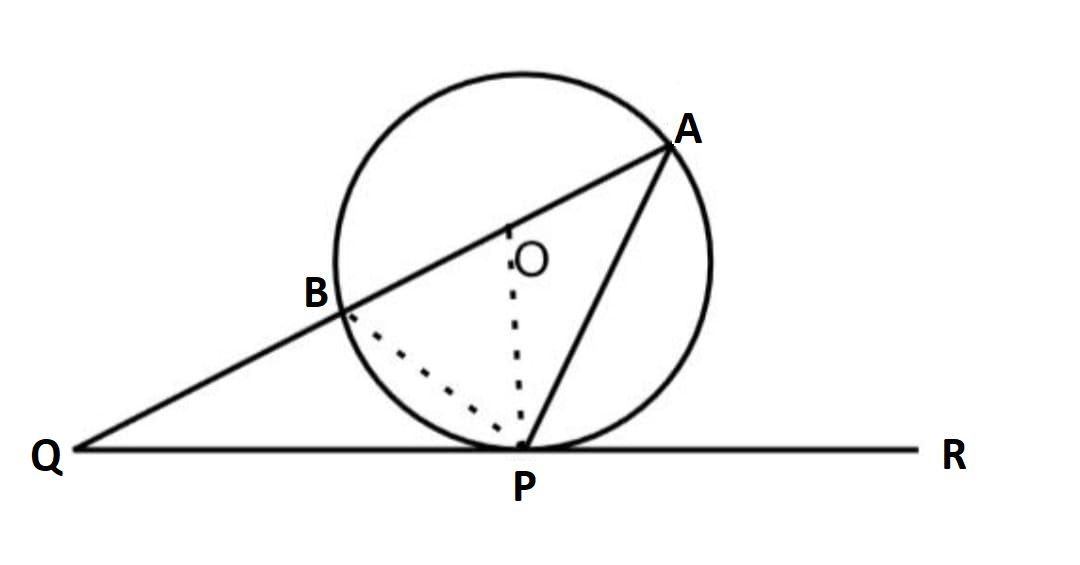
\includegraphics[width=\columnwidth]{figs/circle8.jpg}
			\caption{}
			\label{fig:circle8}
		\end{figure}
	\item In the given figure \figref{fig:circle9}, $ TA $ is a tangent to the circle with centre $ \vec{O} $ such that $ OT = 4 cm , \angle{OTA} = 30{\degree} $, then length of $ TA $ is :
		\begin{figure}[H]
			\centering
			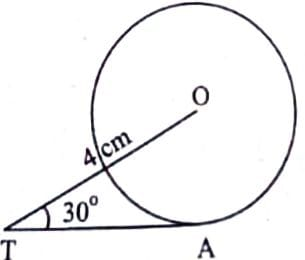
\includegraphics[width=\columnwidth]{figs/circle9.jpg}
			\caption{}
			\label{fig:circle9}
		\end{figure}
		\begin{enumerate}
			\item $ 2\sqrt{3} cm $
			\item $ 2 cm $
			\item $ 2\sqrt{2} cm $
			\item $ \sqrt{3} cm $
		\end{enumerate}
	\item In the given figure \figref{fig:circle10}, $ PT $ is a tangent at $ \vec{T} $ to the circle with centre $ \vec{O} $. If $ \angle{TPO} = 25{\degree} $, then $ x $ is equal to : 	
		\begin{figure}[H]
			\centering
			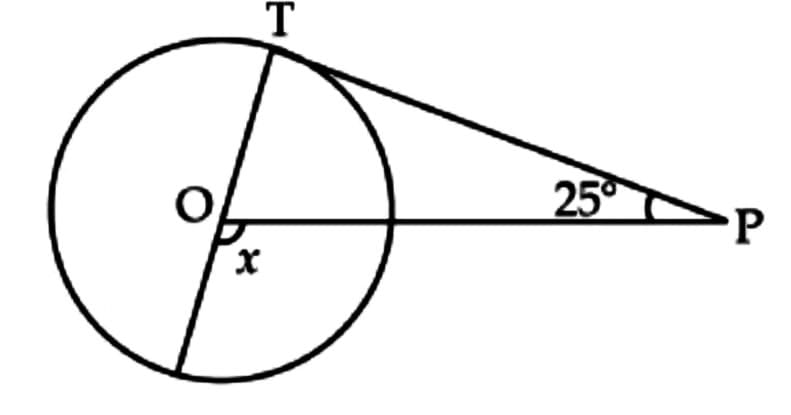
\includegraphics[width=\columnwidth]{figs/circle10.jpg}
			\caption{}
			\label{fig:circle10}
		\end{figure}
		\begin{enumerate}
			\item $ 25{\degree} $
			\item $ 65{\degree} $
			\item $ 90{\degree} $
			\item $ 115{\degree} $
		\end{enumerate}
	\item Two concentric circles are of radii 5 cm and 3 cm. Find the length of the chord of the larger circle which touches the smaller circle.
\end{enumerate}

